\documentclass[a4paper]{article}
\usepackage[landscape]{geometry}
\usepackage[utf8]{inputenc}
\usepackage{url}
\usepackage{multicol}
\usepackage{amsmath}
\usepackage{esint}
\usepackage{amsfonts}
\usepackage{tikz}
\usetikzlibrary{decorations.pathmorphing}
\usepackage{amsmath,amssymb}
\usepackage{fourier}

% mine
\usepackage[colorlinks]{hyperref}
\usepackage{booktabs}
\providecommand{\tightlist}{%
  \setlength{\itemsep}{0pt}\setlength{\parskip}{0pt}}

\usepackage{colortbl}
\usepackage{xcolor}
\usepackage{mathtools}
\usepackage{amsmath,amssymb}
\usepackage{enumitem}
\usepackage{circuitikz}
\makeatletter

\newcommand*\bigcdot{\mathpalette\bigcdot@{.5}}
\newcommand*\bigcdot@[2]{\mathbin{\vcenter{\hbox{\scalebox{#2}{$\m@th#1\bullet$}}}}}
\newcommand{\rsh}{\rotatebox[origin=c]{180}{$\Lsh$}}
\makeatother

\title{ITE Cheat Sheet}
\usepackage[ngerman]{babel}
\usepackage[utf8]{inputenc}

\advance\topmargin-.8in
\advance\textheight3in
\advance\textwidth3in
\advance\oddsidemargin-1.5in
\advance\evensidemargin-1.5in
\parindent0pt
\parskip2pt
\newcommand{\hr}{\centerline{\rule{3.5in}{1pt}}}
%\colorbox[HTML]{e4e4e4}{\makebox[\textwidth-2\fboxsep][l]{texto}
\begin{document}

\begin{center}{\huge{\textbf{CS:Technical::Electrical}}}\\
\end{center}
\begin{multicols*}{3}

\tikzstyle{mybox} = [draw=black, fill=white, very thick,
    rectangle, rounded corners, inner sep=10pt, inner ysep=10pt]
\tikzstyle{fancytitle} =[fill=black, text=white, font=\bfseries]


%! this section is not complete

%------------ Prefixes ---------------
\begin{tikzpicture}
  \node [mybox] (box){%
      \begin{minipage}{0.3\textwidth}

      \end{minipage}
  };
  %------------ Prefixes Header ---------------------
  \node[fancytitle, right=10pt] at (box.north west) {Unit prefixes};
\end{tikzpicture}

%------------ Prefixes ---------------
\begin{tikzpicture}
  \node [mybox] (box){%
      \begin{minipage}{0.3\textwidth}
        \begin{tabular}{@{}lll@{}}
          \toprule
          symbol & name & factor \\
          \midrule
          
          \(T\) & tera & \(\cdot 10^{12}\) \\
          \(G\) & giga & \(\cdot 10^{9}\) \\
          \(M\) & mega & \(\cdot 10^{6}\) \\
          \(k\) & kilo & \(\cdot 10^{3}\) \\
          & 1 & \(\cdot 10^{0}\) \\
          \(m\) & milli & \(\cdot 10^{-3}\) \\
          \(\mu\) & mikro & \(\cdot 10^{-6}\) \\
          \(n\) & nano & \(\cdot 10^{-9}\) \\
          \(p\) & piko & \(\cdot 10^{-12}\) \\
          \(f\) & femto & \(\cdot 10^{-15}\) \\
          \(a\) & atto & \(\cdot 10^{-18}\) \\
          \bottomrule
          \end{tabular}
      \end{minipage}
  };
  %------------ Prefixes Header ---------------------
  \node[fancytitle, right=10pt] at (box.north west) {Unit prefixes};
\end{tikzpicture}

\renewcommand\labelitemi{}
\renewcommand\labelitemii{\rotatebox[origin=c]{180}{$\Lsh$}}

%------------ Prefixes ---------------
\begin{tikzpicture}
  \node [mybox] (box){%
      \begin{minipage}{0.3\textwidth}
        test
        \begin{itemize}[leftmargin=*]
          \tightlist
          \item
            Charge is a property of elementary particles
          
            \begin{itemize}[leftmargin=*]
            \tightlist
            \item
              electrons, protons, pions, muons,
            \item
              there is positive and negative charge
            \item
              charge occurs only in discrete units
            \item
              some particles don't have charge (neutrons, photons,\ldots)
            \end{itemize}
          \item
            The unit for charge is the coulomb \(C\)
          \item
            The unit load is \(e=1.602176634\cdot 10^{-19}C\)
          \item
            One coulomb requires about \(6.25\cdot 10^{18}\) electrons
          \item
            Analogy for charge is amount of water (litres, kg)
          \end{itemize}
      \end{minipage}
  };
  %------------ Prefixes Header ---------------------
  \node[fancytitle, right=10pt] at (box.north west) {Charge};
\end{tikzpicture}



\begin{center}\rule{0.5\linewidth}{0.5pt}\end{center}

\hypertarget{current}{%
\subsection{Current}\label{current}}

\begin{itemize}
\tightlist
\item
  Current (symbol usually \(I\)) is the flow of charge \(Q\), i.e
  charge per time: \(I=Q/T\) or, more precisely, \(I=dQ/dt\)
\item
  The unit for current is ampere \(A\)
\item
  At \(1 A\), \(1\) coulomb flows through a wire per second
\item
  Analogy for current is water flow (litres/second)
\end{itemize}

--

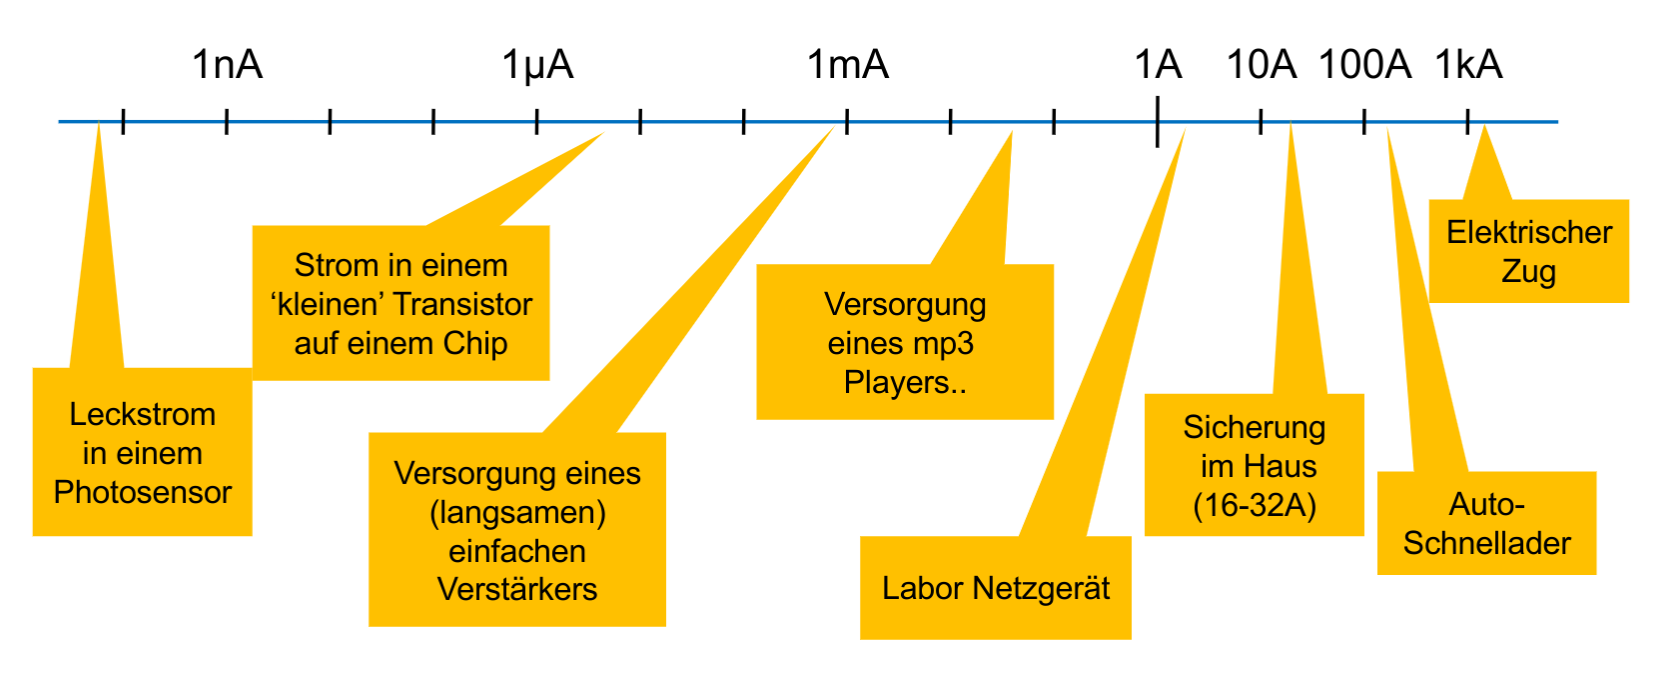
\includegraphics{../assets/images/2022-02-06-20-42-18.png}

\begin{center}\rule{0.5\linewidth}{0.5pt}\end{center}

\hypertarget{voltage}{%
\subsection{Voltage}\label{voltage}}

\begin{itemize}
\tightlist
\item
  Voltage is the difference in electrical potentials

  \begin{itemize}
  \tightlist
  \item
    i.e.~the energy required to move a unit charge in an electric field
  \end{itemize}
\item
  the unit for voltage is volt \(V\)
\item
  Analogy for voltage is water level / pressure (Pa)
\end{itemize}

--

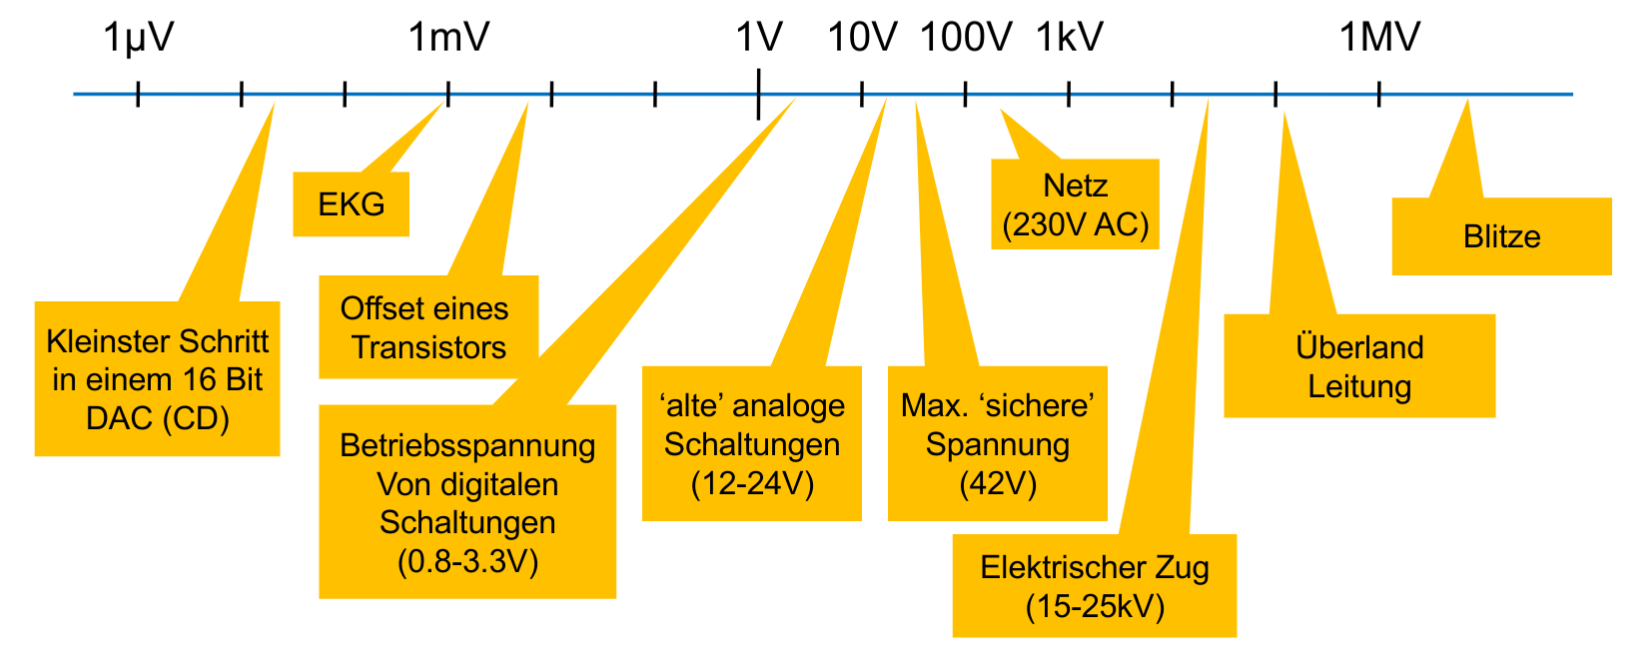
\includegraphics{../assets/images/2022-02-06-20-46-22.png}

\begin{center}\rule{0.5\linewidth}{0.5pt}\end{center}

\hypertarget{ground}{%
\subsection{Ground}\label{ground}}

\begin{itemize}
\tightlist
\item
  Ground is a reference potential to which we relate all voltages
\item
  A synonym for ground is mass
\item
  switch symbols are:
  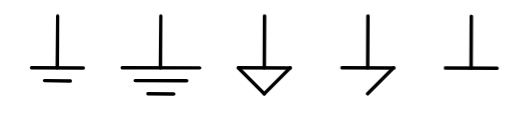
\includegraphics{../assets/images/2022-02-06-20-55-45.png}
\end{itemize}

\begin{center}\rule{0.5\linewidth}{0.5pt}\end{center}

\hypertarget{kirchhoffs-laws}{%
\subsection{Kirchhoff's laws}\label{kirchhoffs-laws}}

\begin{itemize}
\tightlist
\item
  node rule: The sum of all currents in a node is zero
  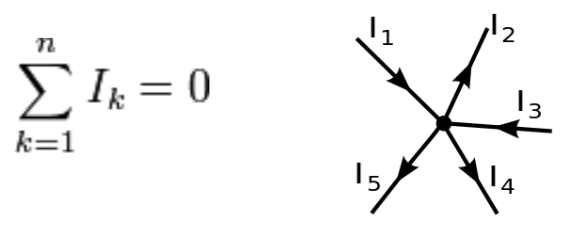
\includegraphics{../assets/images/2022-02-06-21-02-31.png} Follows from
  conservation of charge (charge cannot vanish).
\end{itemize}

--

\begin{itemize}
\tightlist
\item
  loop rule: The sum of the voltages in a closed loop is zero
  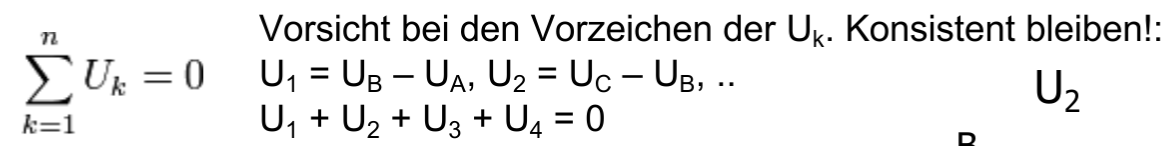
\includegraphics{../assets/images/2022-02-06-21-04-47.png} Follows from
  conservation of energy
\end{itemize}

\begin{center}\rule{0.5\linewidth}{0.5pt}\end{center}

\hypertarget{power}{%
\subsection{Power}\label{power}}

\begin{itemize}
\tightlist
\item
  In order to maintain a current flow, energy must be constantly
  expended.
\item
  The required power is \(P=U\cdot I\)
\item
  The unit for power is \(W\) watt
\end{itemize}

\begin{center}\rule{0.5\linewidth}{0.5pt}\end{center}

\hypertarget{energy}{%
\subsection{Energy}\label{energy}}

\begin{itemize}
\tightlist
\item
  The (electric) energy is \(E=P\cdot T\) (power over time)
\item
  The unit for energy is \(J\) joule
\item
  A full car `battery' (accumulator) contains e.g.~an energy of
  \(50 kWh = 50 kW \cdot 1h = 50,000 W \cdot 3,600 s = 180 MJ\)
\end{itemize}

\begin{center}\rule{0.5\linewidth}{0.5pt}\end{center}

\hypertarget{resistors}{%
\subsection{Resistors}\label{resistors}}

\begin{itemize}
\tightlist
\item
  A resistor is a component with 2 terminals that a current can flow
  through if a voltage is applied
\item
  The unit for resistance is \(\Omega\) omega
\item
  If the current is proportional to the voltage, we call it ohmic
  resistor that holds:

  \begin{itemize}
  \tightlist
  \item
    \(I=U\cdot G\), \(\;G\) is the master value in Siemens \([S]\)
  \item
    \(I=U/R\), \(\;R\) is the resistance in ohm \([\Omega]\)
  \item
    \(G, R\) describe the same behavior. \(G = 1/R, R = 1/G\)
  \end{itemize}
\item
  Switch symbols are:
  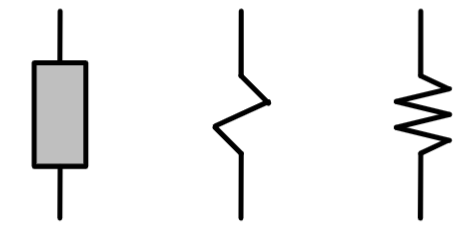
\includegraphics{../assets/images/2022-02-06-21-28-06.png}
\end{itemize}

--

\begin{itemize}
\tightlist
\item
  Parallel connection of resistors
  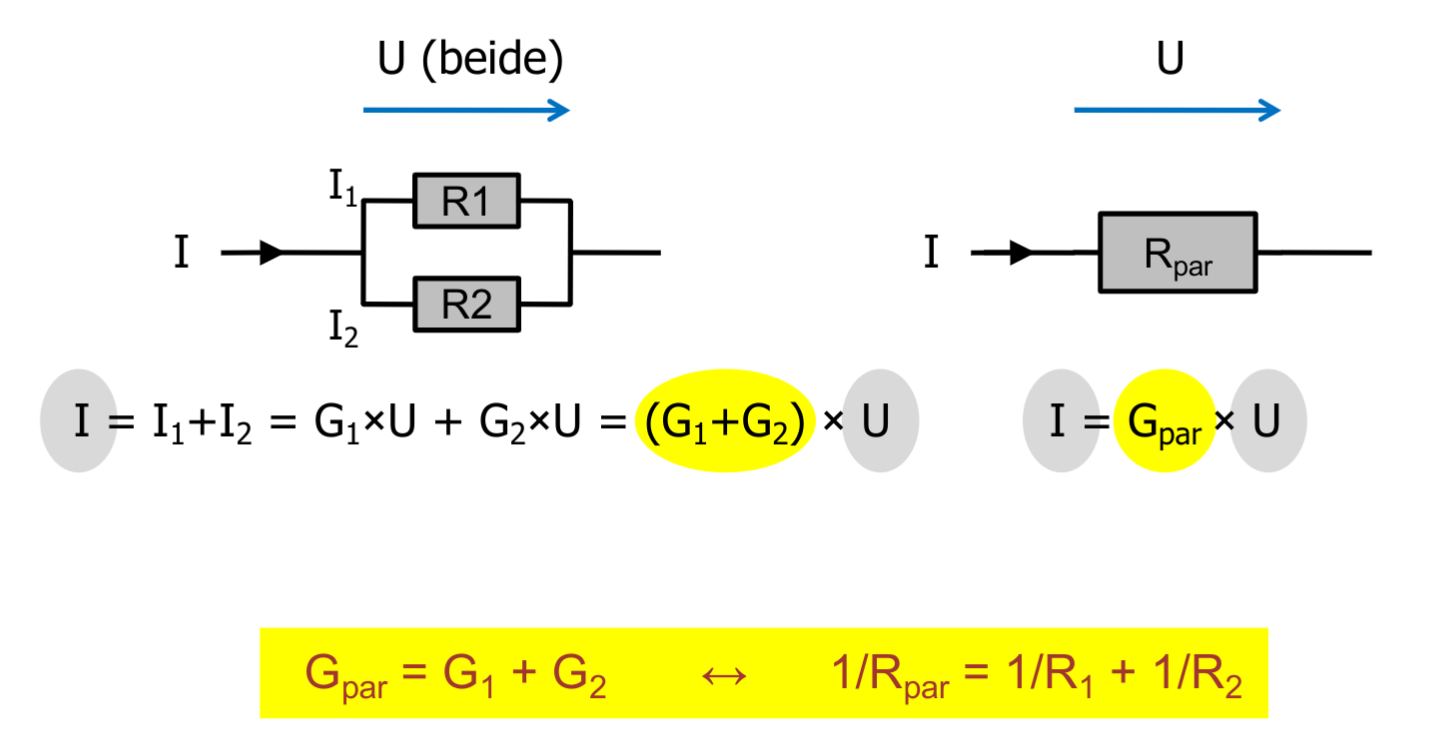
\includegraphics{../assets/images/2022-02-06-21-31-37.png}
\end{itemize}

--

\begin{itemize}
\tightlist
\item
  Series connection of resistors
  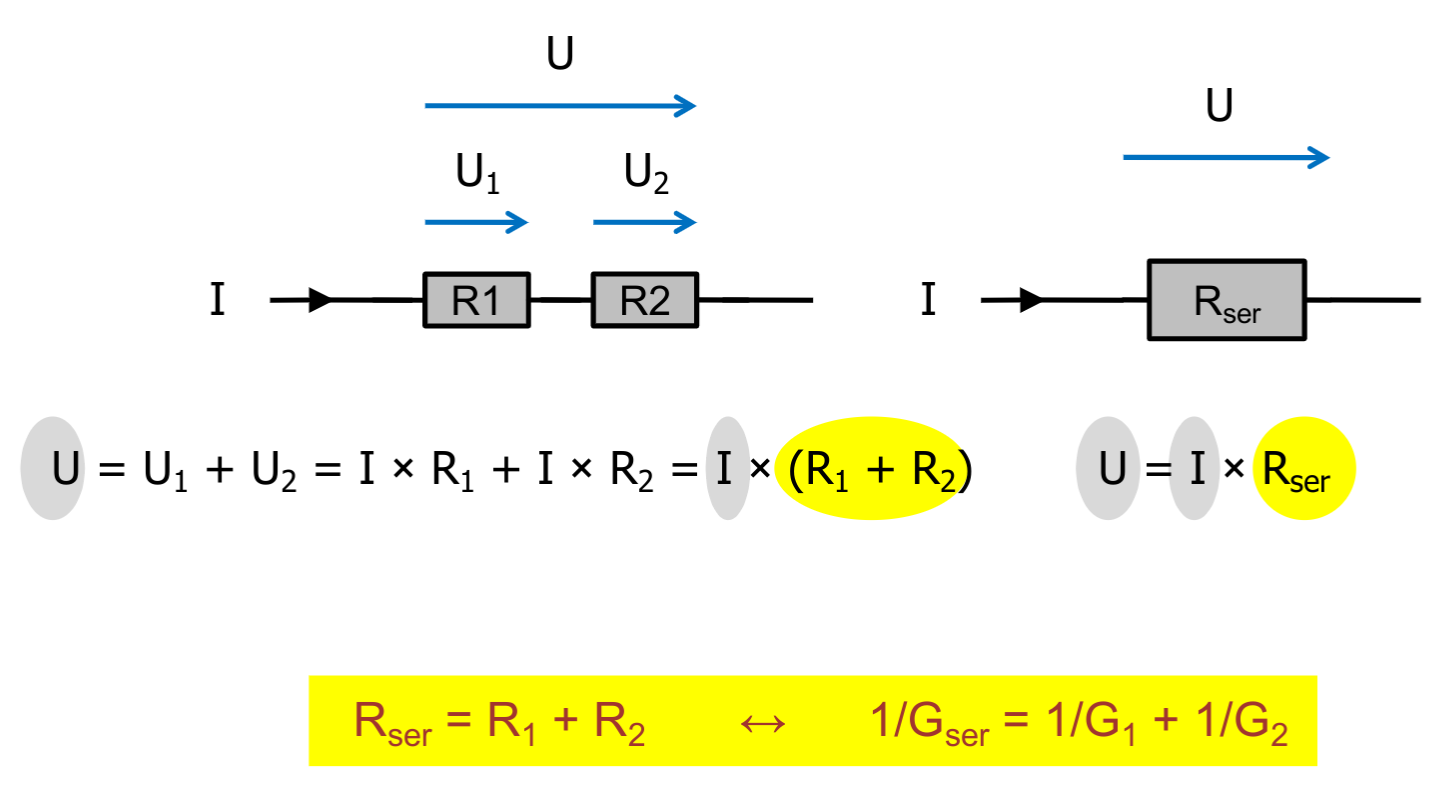
\includegraphics{../assets/images/2022-02-06-21-32-56.png}
\end{itemize}

\begin{center}\rule{0.5\linewidth}{0.5pt}\end{center}

\hypertarget{voltage-divider}{%
\subsection{Voltage Divider}\label{voltage-divider}}

\[
\begin{circuitikz} \draw
(0,0) to[battery] (0,4)
  to[ammeter] (4,4) -- (4,0)
  to[lamp] (0,0);
\end{circuitikz}
\]

\begin{center}\rule{0.5\linewidth}{0.5pt}\end{center}

\hypertarget{capacitors-capacitance}{%
\subsection{Capacitors / Capacitance}\label{capacitors-capacitance}}

\begin{itemize}
\tightlist
\item
  A capacitor can store charge (Q).
\item
  The unit for capacity is \(C\) farad
\item
  The capacity is \(C=Q/U\)
\item
  Analogy for capacitor is bathtub holding water level
\item
  Charge capacitor

  \begin{itemize}
  \tightlist
  \item
    without resistor: \(U(t) = \frac{I_0}{C}\cdot t\)
  \item
    with resistor \(U(t) = U_0 - U_0 e^{-\frac{t}{RC}}\)
  \end{itemize}
\end{itemize}

\end{multicols*}
\end{document}
